\subsection{Формализация нечёткой величины}

Нечёткая величина X на множестве действительных чисел задаётся функцией принадлежности

\begin{equation}
\mu_X: \mathbb{R}\rightarrow[0,1],
\end{equation}

где значение μ\_X(x) выражает степень принадлежности числа x величине X. Носитель и ядро определяются как

\begin{equation}
\operatorname{supp}X=\{x\mid \mu_X(x)>0\},\qquad \operatorname{core}X=\{x\mid \mu_X(x)=1\}.
\end{equation}

Для $\alpha\in[0,1]$ $\alpha$-срез имеет вид

\begin{equation}
X_\alpha=\{x\in\mathbb{R}\mid \mu_X(x)\geq\alpha\}.
\end{equation}

Для нормальной выпуклой величины каждый срез является отрезком [L(α),R(α)]. Вложенность срезов выражается условием

\begin{equation}
\alpha_1<\alpha_2 \Rightarrow X_{\alpha_2}\subseteq X_{\alpha_1},
\end{equation}

что в дискретном представлении проверяется неубыванием левых границ и неувеличением правых границ. Теорема о декомпозиции позволяет восстановить функцию принадлежности по семейству срезов:

\begin{equation}
\mu_X(x)=\sup\{\alpha\mid x\in X_\alpha\}.
\end{equation}

В структуре \texttt{fz\_number} это семейство хранится в векторах \texttt{left} и \texttt{right}. Для исходной величины дополнительно сохраняются \texttt{uniform}, \texttt{a} и \texttt{b}, что позволяет использовать точные формулы без обращения к дискретной сетке.

\subsection{Равномерный закон U(a,b) как исходная нечёткая величина}

Для a<b равномерное распределение задаётся плотностью

\begin{equation}
f(x)= \begin{cases} \frac{1}{b-a}, & a\leq x\leq b,\\ 0, & \text{иначе}. \end{cases}
\end{equation}

В проекте в качестве функции принадлежности используется нормированная линейная функция на том же носителе:

\begin{equation}
\mu_{U(a,b)}(x)= \begin{cases} \frac{x-a}{b-a}, & a\leq x\leq b,\\ 0, & \text{иначе}. \end{cases}
\end{equation}

Она возрастает от нуля в точке a до единицы в точке b. Носитель равен [a,b], ядро — одноточечное множество \{b\}. На уровне α левая граница определяется как

\begin{equation}
L(\alpha)=a+\alpha(b-a),
\end{equation}

а правая граница постоянна:

\begin{equation}
R(\alpha)=b.
\end{equation}

Следовательно,

\begin{equation}
U(a,b)_\alpha=[a+\alpha(b-a),b], \quad |U(a,b)_\alpha|=(1-\alpha)(b-a).
\end{equation}

В \texttt{make\_uniform} эта зависимость вычисляется для всех \texttt{levels} значений сетки α\_i=i/(m−1). Для U(a,b) дискретизация не вносит аппроксимационной ошибки в положение левой границы, так как функция L(α) линейна. Для результатов операций срез на промежуточном уровне получают линейной интерполяцией.

Центр тяжести исходной величины вычисляется аналитически:

\begin{equation}
c_X=\frac{\int_a^b x\mu_X(x)\,dx}{\int_a^b\mu_X(x)\,dx} =a+\frac{2}{3}(b-a).
\end{equation}

Для величин общего вида \texttt{fz\_centroid} применяет численное интегрирование по 2000 равным шагам с трапецеидальными весами. Если площадь под функцией принадлежности вырождается, возвращается середина носителя.

\subsection{Концепция α-уровней в кластеризации}

α-срез переводит нечёткое число в интервал, который содержит значения с принадлежностью не ниже выбранного порога. При α=0 анализируется полный носитель. При α=1 для U(a,b) срез вырождается в точку b. Таким образом, увеличение α уменьшает неопределённость и смещает левую границу к правой.

Для каждого элемента набора на фиксированном α формируется пара

\begin{equation}
P_i=(A_i,B_i)=(L_i(\alpha),R_i(\alpha)).
\end{equation}

Кластеризация выполняется на этих парах. Геометрическое расстояние между отрезками определяется формулой

\begin{equation}
d_i= d([A_1,B_1],[A_2,B_2])= \max\left(|A_1-A_2|,|B_1-B_2|\right).
\end{equation}

Эта функция совпадает с расстоянием Хаусдорфа для компактных интервалов на прямой. Представление P\_i на плоскости делает левую границу координатой x, а правую границу координатой y. Центр кластера является парой средних координат

\begin{equation}
C_j=\left(\frac{1}{n_j}\sum_{i\in K_j}A_i, \frac{1}{n_j}\sum_{i\in K_j}B_i\right).
\end{equation}

Разброс кластера вычисляется как среднеквадратичное расстояние:

\begin{equation}
s_j=\sqrt{\frac{1}{n_j}\sum_{i\in K_j}d(P_i,C_j)^2}.
\end{equation}

Поэтому центр и разброс имеют непосредственную интерпретацию в единицах исходной величины. Веб-интерфейс выводит точки (A,B), центры кластеров и отрезки, окрашенные по меткам.

\begin{figure}[htbp]\centering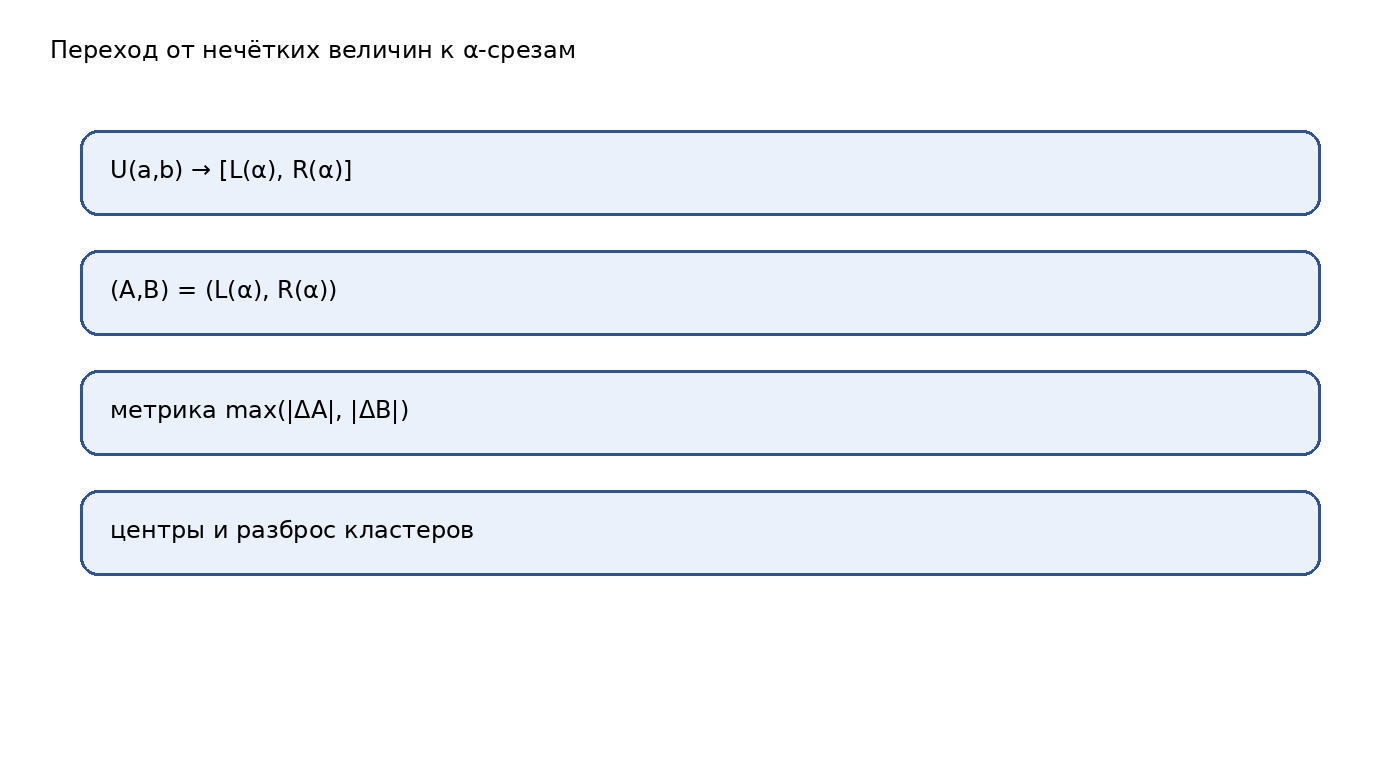
\includegraphics[width=0.9\textwidth]{figures/fig2_alpha.png}\caption{распределение α-срезов на плоскости (A,B)}\label{fig:2}\end{figure}

\subsection{Интервальная арифметика по принципу обобщения Заде}

Для непрерывной монотонной операции принцип обобщения Заде реализуется вычислением образа α-срезов. Пусть X\_α=[x\_1,x\_2], Y\_α=[y\_1,y\_2]. Тогда

\begin{equation}
(X+Y)_\alpha=[x_1+y_1,x_2+y_2],
\end{equation}

\begin{equation}
(X-Y)_\alpha=[x_1-y_2,x_2-y_1].
\end{equation}

Для произведения вычисляются четыре комбинации границ:

\begin{equation}
(XY)_\alpha=[\min P,\max P], \quad P=\{x_1y_1,x_1y_2,x_2y_1,x_2y_2\}.
\end{equation}

Для деления при $0\notin\operatorname{supp}Y$ используется умножение на обратный интервал:

\begin{equation}
(X/Y)_\alpha=X_\alpha\cdot[1/y_2,1/y_1].
\end{equation}

В \texttt{combine} сетка результата выбирается как максимум числа уровней двух операндов. На каждом уровне исходные срезы извлекаются через \texttt{cut\_at}, затем выполняется соответствующая операция. После этого для каждого i>0 левая граница заменяется на max(L\_i,L\_\{i−1\}), а правая — на min(R\_i,R\_\{i−1\}). Шаг восстанавливает вложенность при накоплении численной погрешности.

Деление с носителем делителя, содержащим ноль, блокируется в \texttt{fz\_apply}. Ошибка сохраняется в thread-local строке \texttt{g\_error}, а вызывающая сторона получает \texttt{NULL}. Это предотвращает формирование неограниченного или разрывного результата в модели, рассчитанной на конечные вложенные интервалы.

\subsection{Сравнение нечётких величин}

Сравнение возвращает знак разности центров тяжести:

\begin{equation}
\operatorname{cmp}(X,Y)=\operatorname{sign}(c_X-c_Y),
\end{equation}

при этом используется масштабируемый допуск

\begin{equation}
\varepsilon=10^{-9}\max(1,|c_X|,|c_Y|).
\end{equation}

Одновременно вычисляется степень возможности

\begin{equation}
\operatorname{Poss}(X\geq Y)= \sup_{u\geq v}\min(\mu_X(u),\mu_Y(v)).
\end{equation}

В дискретной реализации на общей сетке уровней проверяется условие R\_X(α)≥L\_Y(α), и максимальный подходящий α записывается в \texttt{degree}. В Go-слое операция сравнения выполняется в обоих направлениях, поэтому клиент получает \texttt{Poss(X≥Y)} и \texttt{Poss(Y≥X)}.

\subsection{Генерация случайных наборов}

В \texttt{rng.cpp} состояние xoshiro256** состоит из четырёх 64-битных слов. Инициализация выполняется четырьмя последовательными вызовами splitmix64 от исходного seed. Следующее состояние использует XOR-сдвиги и циклическую перестановку \texttt{rotl}, а выходное значение вычисляется как \texttt{rotl(s[1]*5,7)*9}.

Преобразование в число из [0,1) имеет вид

\begin{equation}
u=(x\mathbin{\gg}11)2^{-53}.
\end{equation}

Для генерации элемента выбираются

\begin{equation}
a\sim U[lo,hi],\qquad w\sim U[w_{min},w_{max}],\qquad b=a+w.
\end{equation}

\texttt{fz\_set\_generate} резервирует память под n элементов, создаёт величины через \texttt{make\_uniform} и записывает параметры генерации в журнал. Проверяются ограничения n∈[1,100000], lo≤hi и 0<w\_min≤w\_max.

\subsection{Отбор и кластеризация}

Отбор по ширине оставляет индексы, для которых

\begin{equation}
w_{min}\leq B_i-A_i\leq w_{max}.
\end{equation}

Отбор по окну оставляет интервалы, удовлетворяющие

\begin{equation}
x_1\leq A_i,\qquad B_i\leq x_2.
\end{equation}

В \texttt{selection.cpp} обе операции выполняют один линейный проход и записывают исходные индексы в пользовательский массив.

Алгоритм k-means++ принимает k и seed. Первый центр выбирается случайно. Для каждого следующего центра строится распределение вероятностей, пропорциональное квадрату расстояния до ближайшего выбранного центра. Затем выполняются назначение к ближайшему центру и пересчёт средних границ. Пустой кластер заполняется наиболее удалённым объектом. Цикл ограничен параметром \texttt{max\_iter}, а Go-обёртка передаёт 300 итераций.

Пороговый алгоритм не требует заранее заданного k. Сначала интервалы сортируются по A, затем последовательно относятся к ближайшему центру, если расстояние не превышает δ. Иначе создаётся новый кластер. Далее выполняется до 50 уточняющих проходов с переназначением объектов и пересчётом центров. После стабилизации метки перенумеровываются в порядке возрастания A.

---
